\documentclass[12pt, a4paper]{article}
\usepackage[utf8]{inputenc}
\usepackage{graphicx}
\usepackage[portuguese]{babel}
\usepackage{amsmath, amssymb}
\usepackage[hidelinks]{hyperref}
\usepackage{geometry}
\usepackage{float}
\geometry{margin=1in}

\title{Trabalho final de Computação Reconfigurável}
\author{Alexandre André Neves Pita\\
Instituto Superior de Engenharia \\
Universidade do Algarve \\}
\date{\today}

\begin{document}

\begin{titlepage}
    \centering
    \vspace*{2cm}

    {\Large\textbf{Universidade do Algarve}}\\[1.5cm]

    {\Huge\textbf{Trabalho final de Computação Reconfigurável}}\\[2cm]

    {\Large Alexandre André Neves Pita}\\
    74526\\[1.5cm]

    {\large Curso de Engenharia de Sistemas e Tecnologicas Informáticas}\\
    Instituto Superior de Engenharia\\[2cm]

    {\large \today}

    \vfill
\end{titlepage}
\pagenumbering{roman} % Use Roman numerals for TOC and front matter
\newpage
\tableofcontents
\newpage

\pagenumbering{arabic} % Switch to normal numbering

\section{Introdução}
O Trabalho Final da unidade curricular de Computação Reconfigurável tem como principal objetivo o desenvolvimento de um projeto que integre diversos componentes de hardware reconfigurável,
 implementados em VHDL, os quais foram previamente concebidos ao longo dos trabalhos realizados durante o semestre.
Este projeto pretende consolidar os conhecimentos adquiridos, promovendo a aplicação prática dos mesmos, e explorar a interligação e o controlo conjunto de vários módulos.\\
\\
O procedimento deste trabalho consiste na filtragem de um sinal com ruído, com o objetivo de obter um sinal mais limpo.\\  
Antes de ser transmitida, a informação proveniente do sinal ruídoso é processada por um módulo de encriptação, que assegura a proteção dos dados durante a transmissão.\\
De seguida, a informação encriptada é enviada para um módulo UART, responsável pela transmissão em série para o "Controller2".\\
No "Controller2", essa mesma informação é recebida por outro módulo UART, que converte os dados de formato série para paralelo, permitindo o seu encaminhamento para o módulo de desencriptação.\\
Após o processo de desencriptação, procede-se à filtragem do sinal, utilizando os coeficientes armazenados na ROM do "Controller2", onde se encontra o filtro. Os dados resultantes da filtragem são posteriormente guardados num ficheiro de texto.\\


A imagem apresentada em seguida ilustra a arquitetura simplificada do sistema proposto para este trabalho.\\

\begin{figure}[h]  % 'h' means "here" (placement)
    \centering
    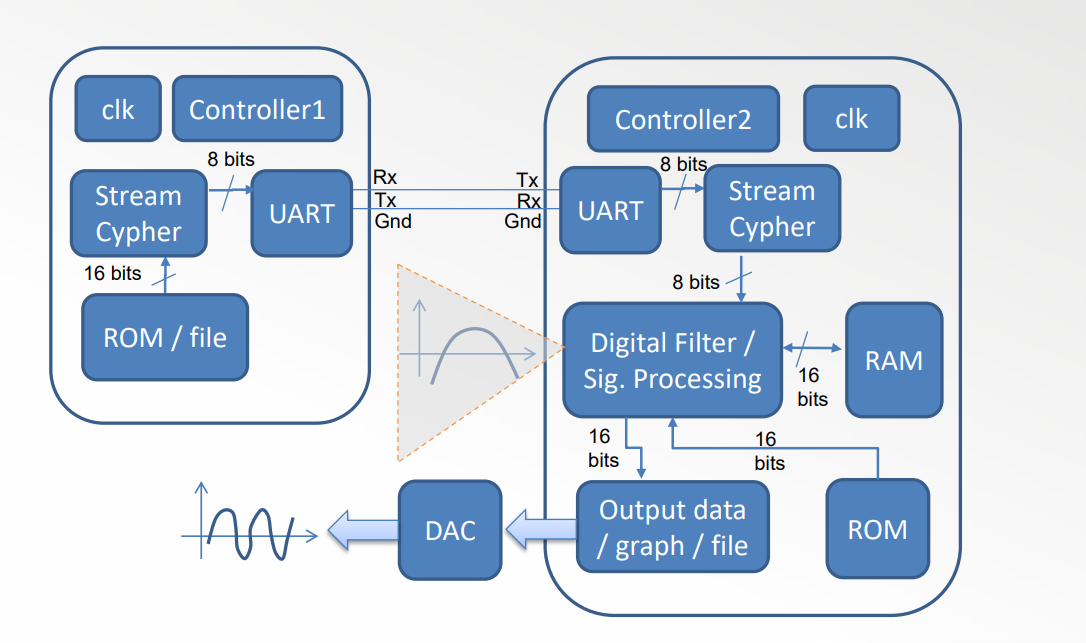
\includegraphics[width=0.6\textwidth]{./images/architecture.png}  % adjust width or use height=
    \caption{Arquitetura do sistema proposto.}
    \label{fig:arquitetura}
\end{figure}

Ao observar a imagem, é possível identificar dois controladores, designadamente o "Controller1" e o "Controller2". \\ \\
No interior do "Controller1" encontram-se vários módulos, descritos na lista abaixo:

\begin{itemize}
    \item \textbf{Módulo ROM / File:} Módulo que contém informação acessível por outros componentes.  
    Neste projeto, foi utilizada uma ROM para armazenamento dos dados correspondentes ao sinal com ruído.
    
    \item \textbf{Módulo Cypher:} Responsável pela encriptação da mensagem proveniente da ROM.
    
    \item \textbf{Módulo UART:} Encarregado de transmitir, de forma sequencial, a informação encriptada para o "Controller2".
\end{itemize}

\vspace{2em} % Adds vertical space between the list and the next paragraph


No "Controller2", também existem vários módulos, que são os seguintes:

\begin{itemize}
    \item \textbf{Módulo UART:} Encarregado de receber, de forma sequencial, a informação encriptada pelo "Controller1".

    \item \textbf{Módulo Cypher:} Responsável pela desencriptação da mensagem proveniente da ROM.
    \item \textbf{Módulo Digital Filter:} Módulo responsável pela filtragem do sinal, que é processado pelo módulo de desencriptação.\\

    \item \textbf{Módulo ROM / File:} Módulo que contém informação acessível por outros componentes.  
    Neste projeto, foi utilizada uma ROM para armazenamento dos dados correspondentes ao filtro.

    \item \textbf{Módulo RAM:} RAM compoenente de escrita e leitura de dados. Neste projeto o mesmo não foi utilizado pois este foi escrito automáticamente para o ficheiro de texto.\\

    \item \textbf{Módulo Output data:} Escrita num ficheiro de texto, com o objetivo de armazenar os dados filtrados.\\
    
\end{itemize}

\newpage

\section{Desenvolvimento do projeto}
Esta secção descreve o desenvolvimento de cada controlador, de forma a garantir uma comunicação eficiente entre os módulos, assegurando a correta correspondência entre as entradas e saídas de cada componente.

\subsection{Controller1}
\subsubsection{Descrição}
O \textit{Controller1} é responsável pela leitura dos dados armazenados numa memória ROM, pela encriptação desses dados e pela sua posterior transmissão em série através de uma interface UART.  
Este módulo foi desenvolvido em VHDL com recurso a uma arquitetura sequencial baseada numa máquina de estados finitos, composta pelos seguintes estados: \texttt{READING}, \texttt{ENCRYPTING}, \texttt{SENDING} e \texttt{DONE}.\\

Inicialmente, os dados são lidos sequencialmente da ROM, onde estão armazenadas amostras de sinal com ruído. Em seguida, cada amostra é submetida a um processo de encriptação bit a bit, através de um módulo \textit{Cypher}.  
A encriptação é realizada em blocos de 8 bits, de modo a que cada grupo de 8 bits seja imediatamente transmitido via UART, sem ser necessário aguardar que os 16 bits da amostra sejam completamente encriptados. Esta abordagem permite reduzir a latência e economizar ciclos de relógio, otimizando o desempenho do sistema.\\

Todo o processo de controlo do \textit{Controller1} é executado na borda descendente do sinal de relógio (\texttt{falling\_edge}), com o objetivo de evitar conflitos de sincronização com os componentes auxiliares (\textit{Cypher} e \textit{UART}), os quais operam na borda ascendente (\texttt{rising\_edge}). Esta escolha permite que os dados estejam disponíveis sem necessitar de esperar um ciclo de relógio adicional, garantindo uma operação mais eficiente.\\

Após a leitura e transmissão de todo o sinal com ruído, o sistema transita para o estado \texttt{DONE}, no qual não são executadas mais operações. O sistema permanece nesse estado até que seja recebido um sinal de reinicialização (\texttt{reset}), que reinicia o processo desde o início.

\subsubsection{Simulação Controller1}
Ao simular apenas o \textit{Controller1}, é possível observar a transição sequencial dos estados da máquina de estados.  
O processo inicia-se no estado \texttt{READING}, onde os dados são lidos da ROM, passando automaticamente para o estado \texttt{ENCRYPTING} no ciclo de relógio seguinte, onde se inicia a encriptação do sinal.  
Observa-se ainda que, após 8 ciclos de relógio, o estado transita para \texttt{SENDING}, uma vez que já foram encriptados 8 bits, quantidade suficiente para serem transmitidos pela interface UART.\\

A imagem abaixo ilustra a simulação realizada no ModelSim, onde são visíveis as transições entre os diferentes estados da máquina de estados, bem como a troca de dados entre os sinais envolvidos no processo.

\begin{figure}[h]
    \centering
    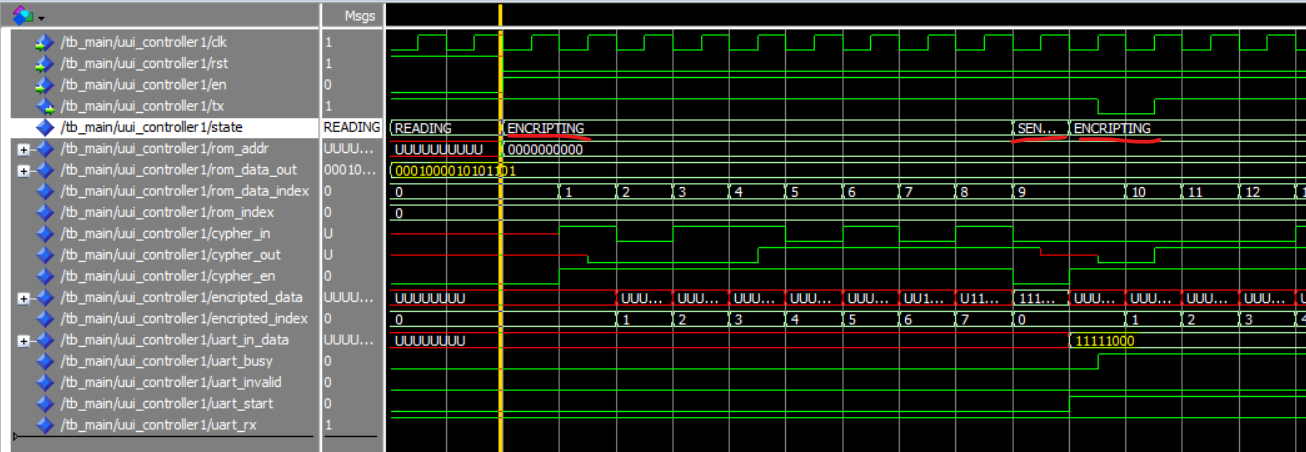
\includegraphics[width=0.95\linewidth]{images/controller1_simulation.png}
    \caption{Simulação no ModelSim do \textit{Controller1} com destaque para os estados e sinais de comunicação.}
    \label{fig:simulacao_controller1}
\end{figure}

\subsubsection{Considerações sobre a Sincronização do Cypher}
É importante destacar que, neste controlador, foi necessário desativar o módulo \textit{cypher} durante os processos de leitura e envio de dados.  
Caso o \textit{cypher} permanecesse ativo nesses momentos, ocorreria uma dessincronização do componente \textit{LFSR} (Linear Feedback Shift Register) presente no seu interior.  
Para que a desencriptação posterior seja bem-sucedida, é essencial que ambos os módulos \textit{cypher} — o de encriptação e o de desencriptação — mantenham a mesma sequência pseudoaleatória, o que implica uma sincronização perfeita dos \textit{LFSRs} com a mesma \textit{seed}.  

Como solução, garantiu-se que o processo de deslocamento (\textit{shift}) do \textit{LFSR} ocorre exclusivamente durante a fase de encriptação.  
Nos restantes estados, o módulo é desativado, impedindo que o \textit{LFSR} continue a avançar, e assim preservando a sincronização necessária para a correta recuperação dos dados encriptados.

Na imagem anterior, é possível observar que o sinal \texttt{cypher\_en} se encontra ativo (em nível lógico '1') durante o estado \texttt{ENCRYPTING}.

\newpage

\subsection{Controller2}
\subsubsection{Descrição}

O \textit{Controller2} é responsável por receber os dados encriptados via UART, realizar a desencriptação bit a bit e aplicar um filtro convolucional aos dados desencriptados. O resultado da convolução é então armazenado para posterior uso ou processamento.  
Este módulo foi desenvolvido em VHDL com uma arquitetura sequencial baseada em uma máquina de estados finitos, composta pelos seguintes estados: \texttt{INIT}, \texttt{DECRIPTING}, \texttt{FILTER} e \texttt{DONE}.\\

O processo começa quando o \textit{Controller2} espera pela receção de dados via UART. Uma vez que os dados são recebidos e o módulo UART está pronto, o controlador transita para o estado de desencriptação (\texttt{DECRIPTING}). Os dados são desencriptados bit a bit utilizando um módulo \textit{Cypher} que opera com um LFSR (Linear Feedback Shift Register), garantindo a reversibilidade da encriptação e a sincronização correta com o emissor dos dados.\\

Após a desencriptação de cada bloco de dados, o controlador acumula as amostras e começa a aplicar o filtro convolucional. O filtro é configurado através de coeficientes armazenados numa ROM. A convolução é realizada com base nas amostras de dados e nos coeficientes do filtro. O resultado da convolução é armazenado no formato apropriado utilizando o módulo \texttt{write\_file}.\\

Este controlador tem como objetivo processar dados encriptados de forma eficiente, realizando operações de desencriptação e filtragem antes de armazenar os resultados. Ele demonstra a capacidade de lidar com sinais ruidosos e a integração de operações de comunicação serial, desencriptação e processamento de sinais, sendo uma solução eficaz para sistemas reconfiguráveis baseados em FPGA.

\subsubsection{Simulação Controller2}
Na simulação é possível identificar duas fases distintas no funcionamento do \textit{Controller2}.\\

\textbf{Fase 1: Receção inicial dos dados}\\

Na primeira fase, o \textit{Controller2} encontra-se a receber os primeiros valores do sinal encriptado enviados pelo \textit{Controller1}. Como o filtro convolucional possui um tamanho de 51 amostras, é necessário aguardar a receção e desencriptação de 51 elementos antes de iniciar o cálculo da convolução. Durante este período, o sistema apenas acumula os dados necessários para que a operação de filtragem seja válida.

\begin{figure}[H]
    \centering
    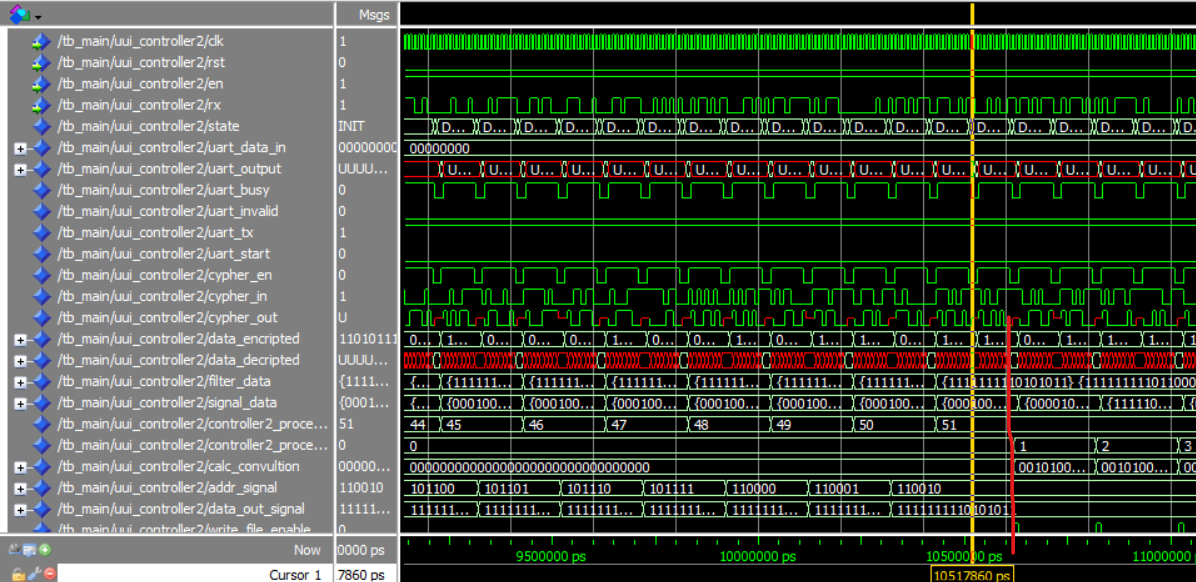
\includegraphics[width=0.9\textwidth]{images/controller2_fase1_simulation.png}
    \caption{Receção e desencriptação inicial dos primeiros 51 valores do sinal.}
    \label{fig:controller2_phase1}
\end{figure}


\textbf{Fase 2: Início da convolução e processamento sequencial}\\

Na segunda fase, com os dados suficientes disponíveis, inicia-se o processo de convolução. A cada novo bloco de 16 bits recebidos, o controlador desencripta os dados e atualiza a janela de amostras, aplicando novamente a convolução com os coeficientes do filtro. Este processo repete-se iterativamente até que todo o sinal tenha sido processado.

\begin{figure}[H]
    \centering
    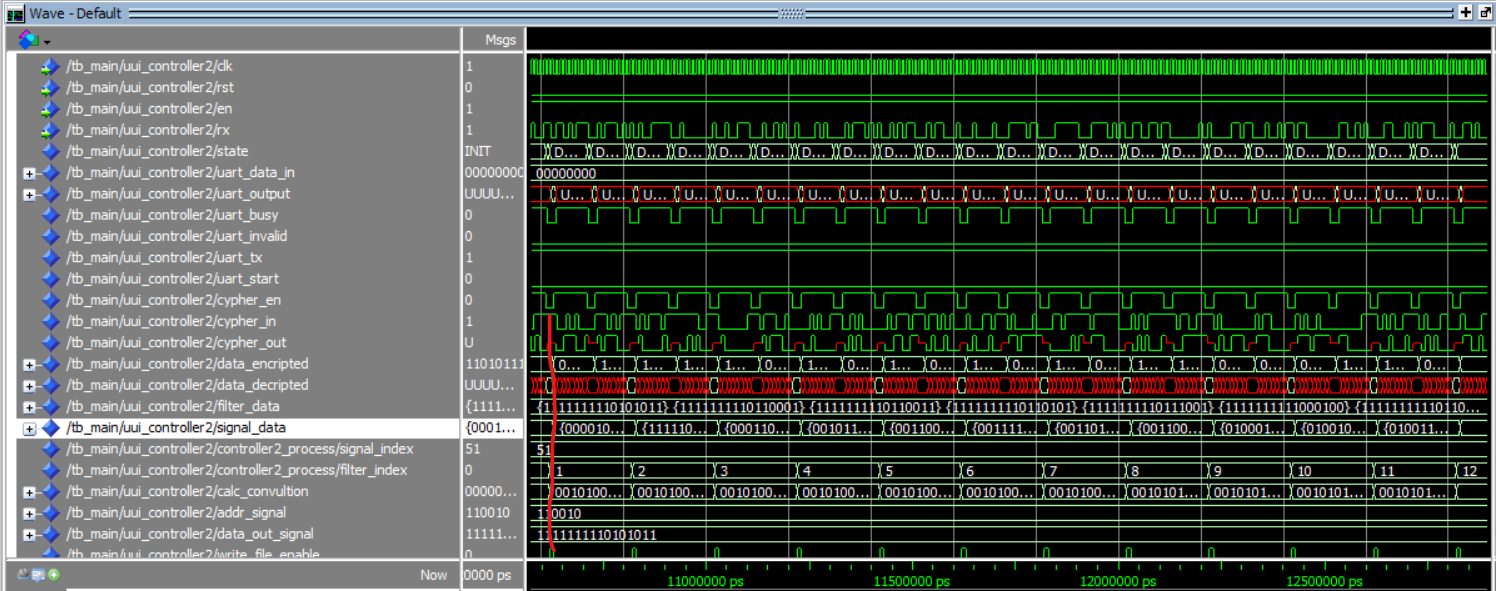
\includegraphics[width=0.9\textwidth]{images/controller2_fase2_simulation.png}
    \caption{Execução contínua da convolução com os dados desencriptados.}
    \label{fig:controller2_phase2}
\end{figure}


\subsubsection{Considerações na otimização do processamento Inicial}

Durante o processo de leitura dos primeiros 51 elementos do sinal, observa-se que os dados são armazenados em registradores internos. Esta abordagem permite que a convolução seja realizada diretamente sobre os dados já disponíveis em memória interna, evitando o acesso repetitivo à ROM a cada nova iteração da janela deslizante.

Esta estratégia resulta numa melhoria significativa de desempenho, uma vez que reduz a latência associada às leituras externas e agiliza o cálculo da convolução.

Após o primeiro cálculo da convolução sobre a janela inicial, o resultado é imediatamente escrito num ficheiro de texto, dando início ao processo contínuo de filtragem do sinal.

\section{Resultados}

Com o sistema implementado e simulado, é possível analisar visualmente os efeitos da filtragem convolucional aplicada ao sinal original com ruído. Esta análise permite verificar a eficácia do processamento realizado pelo \textit{Controller2} após a receção e desencriptação dos dados provenientes do \textit{Controller1}.

Na Figura~\ref{fig:sinal_ruido}, é apresentado o sinal original, previamente armazenado na memória ROM, contendo ruído que simula interferências ou perturbações do ambiente.

\begin{figure}[H]
    \centering
    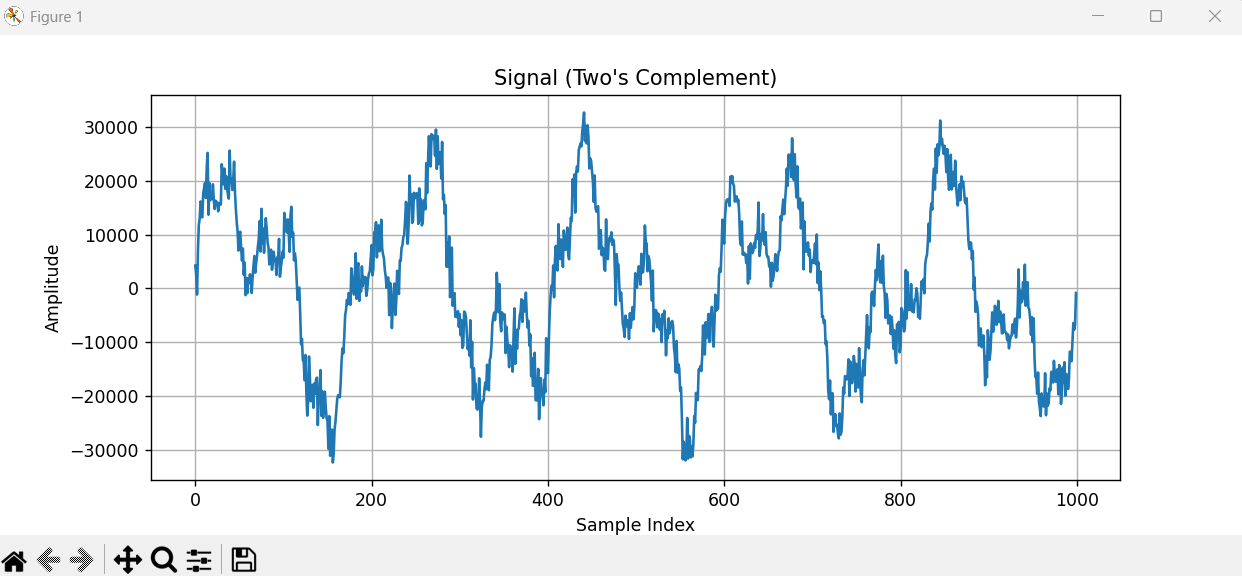
\includegraphics[width=0.85\textwidth]{images/sinal_com_ruido.png}
    \caption{Sinal original com ruído armazenado na ROM.}
    \label{fig:sinal_ruido}
\end{figure}

Após o processamento convolucional com o filtro de 51 coeficientes, observa-se uma atenuação significativa do ruído presente no sinal. O resultado pode ser visualizado na Figura~\ref{fig:sinal_filtrado}, onde é evidente a suavização e recuperação do conteúdo útil do sinal.

\begin{figure}[H]
    \centering
    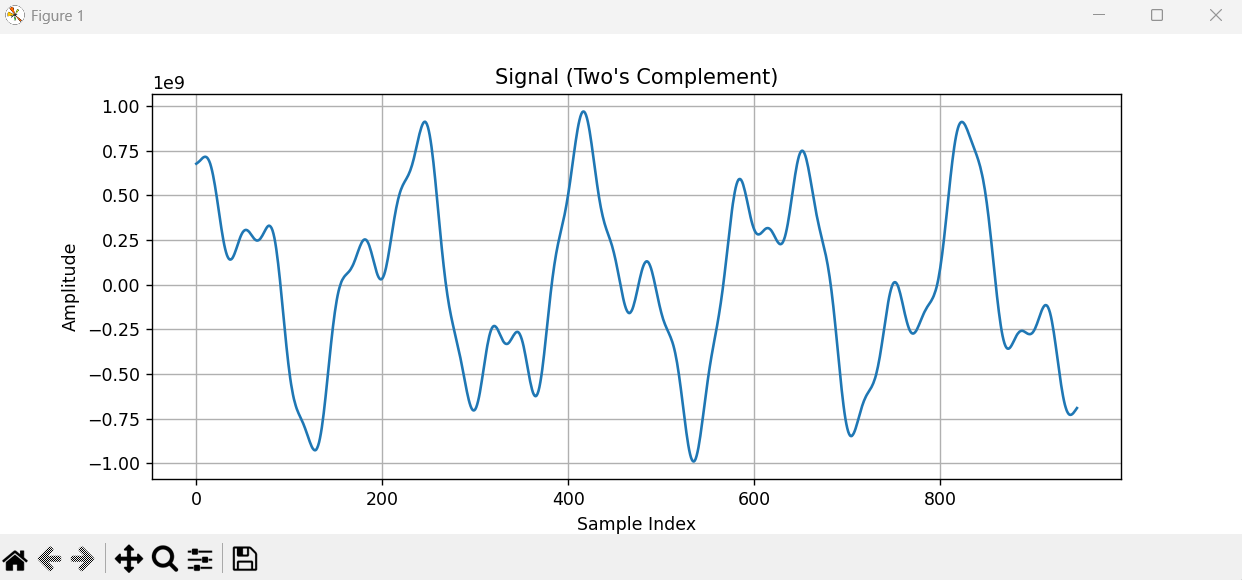
\includegraphics[width=0.85\textwidth]{images/sinal_filtrado.png}
    \caption{Sinal após filtragem: redução de ruído visível.}
    \label{fig:sinal_filtrado}
\end{figure}

Estes resultados demonstram a eficácia do sistema na transmissão segura de dados e na sua subsequente recuperação com filtragem digital, validando os objetivos do projeto e a correta integração de todos os módulos desenvolvidos.


\newpage

\section{Conclusões}

Este trabalho permitiu desenvolver e validar um sistema digital completo, baseado em FPGA, capaz de realizar a transmissão, receção, desencriptação e filtragem de sinais digitais em ambiente simulado.

Ao longo do projeto, foram concebidos dois controladores distintos: o \textit{Controller1}, responsável pela leitura, encriptação e envio dos dados via UART; e o \textit{Controller2}, que realiza a receção, desencriptação e subsequente filtragem convolucional dos dados recebidos. A comunicação entre ambos foi feita utilizando uma ligação serial simples, demonstrando a viabilidade de integração de subsistemas com diferentes funções num ambiente digital sincronizado.

Entre os principais objetivos atingidos destacam-se:
\begin{itemize}
    \item A correta implementação da transmissão de dados encriptados bit a bit;
    \item O desenvolvimento de uma arquitetura sequencial baseada em máquinas de estados finitos, garantindo controlo preciso e sincronizado sobre as operações;
    \item A aplicação eficiente da operação de convolução, recorrendo a buffers circulares para aceleração do processamento;
    \item A escrita dos resultados filtrados para análise posterior, assegurando rastreabilidade e verificação.
\end{itemize}

Para além da consolidação de conhecimentos em VHDL e arquiteturas digitais, este trabalho reforçou competências essenciais na conceção de sistemas síncronos, na utilização de interfaces de comunicação (como UART) e na integração modular de diferentes blocos funcionais.

Futuramente, este projeto poderá ser expandido com suporte a diferentes modos de filtragem, encriptação mais robusta, comunicação bidirecional ou até mesmo a implementação em hardware real para validação em tempo real.

\newpage

\end{document}